\documentclass{beamer}


\usepackage{../macros}

\title{Array}

\begin{document}

\frame{
  \titlepage
}

\begin{frame}[fragile]{Array}
  
  \begin{block}{}
    \begin{itemize}
      \item A collection of items stored at contiguous memory locations
      \item Data structure to store multiple items of the same type
    \end{itemize}
  \end{block}
  
  \begin{block}{}
    \centering
    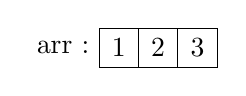
\begin{tikzpicture}[scale = 0.5]
      \draw (0, 0) rectangle (3, 1) 
        (1, 0) -- (1, 1)
        (2, 0) -- (2, 1);
      \draw (0.5, 0.5) node {1};
      \draw (1.5, 0.5) node {2};
      \draw (2.5, 0.5) node {3};
      \draw (0, 0.5) node[left] {arr :};
    \end{tikzpicture}
  \end{block}
  
  \begin{minipage}{0.48\textwidth}
    \begin{code}{In Python}
      \begin{Python}
arr = [1, 2, 3]
      \end{Python}
    \end{code}
    
    \begin{code}{In R}
      \begin{R}
arr <- c(1, 2, 3)
      \end{R}
    \end{code}
  
%    \begin{code}{In Shell}
%      \begin{Shell}
%arr = (1 2 3)
%      \end{Shell}
%    \end{code}
  \end{minipage}\hfill
  \begin{minipage}{0.48\textwidth}
    \begin{code}{In C}
      \begin{C}
int[] arr = {1, 2, 3};
      \end{C}
    \end{code}
  
    \begin{code}{In Java}
      \begin{Java}
int[] arr = {1, 2, 3};
      \end{Java}
    \end{code}
  \end{minipage}
\end{frame}

\begin{frame}{Exercise 1: Making Book}
  \begin{overlayarea}{\textwidth}{\textheight}
  \begin{block}{Statement}
    Given two numbers $A$ and $B$, count the number of occurrences of each digit in the range between $A$ and $B$ included
  \end{block}
  
  \only<2-3|handout:1>{
  \begin{block}{Representation}
    \centering
    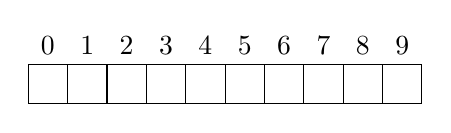
\begin{tikzpicture}[scale = 0.5]
      \draw (0, 0) rectangle (10, 1);
      \foreach \x in {1, 2, ..., 9}
        \draw (\x, 0) -- (\x, 1);
      \foreach \x in {0, 1, ..., 9}
        \draw ({\x + 0.5}, 1) node[above] {\x};
    \end{tikzpicture}
  \end{block}}
  
  \only<3|handout:1>{
  \begin{example}
    \emphv{Input:}\\
      10 15\\
%        15 104\\
%        220 202\\
%        0

        \emphv{Output:}\\
        Case 1: 0:1 1:7 2:1 3:1 4:1 5:1 6:0 7:0 8:0 9:0\\
%        Case 2: 0:14 1:19 2:19 3:19 4:19 5:19 6:19 7:19 8:19 9:19\\
%        Case 3: 0:10 1:11 2:22 3:2 4:2 5:2 6:2 7:2 8:2 9:2
  \end{example}}
  
  \only<4-|handout:2>{
  \begin{block}{What problems can arise?}
    \begin{itemize}
      \item What do we know of $A$ and $B$?
      \item<5-> Can $A > B$?
      \item<6-> Can $A = B$?
      \item<7-> How great can $A$ and $B$ be?
      \item<8-> How great can the number of occurrences be?\\
      \uncover<9->{\emph{$\Longrightarrow$} Are integers big enough for the solution?}\\
      \uncover<10->{\emph{$\Longrightarrow$} What type of array for the solution?}
    \end{itemize}
  \end{block}}
  
  \end{overlayarea}
\end{frame}

\begin{frame}[fragile]{Exercise 1: Making Book}
%  \framesubtitle{Solution 1: Brut force}

  \begin{code}{Solution 1: Brut force}
    \begin{PseudoCode}
read $A$ and $B$ on the standard input
if $A > B$ then 
    exchange their value

initialize the solution array with 0

foreach page between A and B
    foreach digit in page
        increment the corresponding cell

print the result
    \end{PseudoCode}
  \end{code}
\end{frame}

\begin{frame}[fragile]{Exercise 1: Making Book}
%  \framesubtitle{Solution 2: Arithmetic}
  
  \begin{code}{Solution 2: Arithmetic}
    \begin{PseudoCode}
read $A$ and $B$ on the standard input
if $A > B$ then exchange their value

diff $\leftarrow$ $B - A + 1$
initialize the solution array with $\lfloor$diff/10$\rfloor$
    
if diff mod 10 $\neq$ 0 then
    deal with the units
    
A $\leftarrow \lfloor A / 10 \rfloor$
B $\leftarrow \lfloor B / 10 \rfloor$
deal with the tens

print the result
    \end{PseudoCode}
  \end{code}
\end{frame}

\begin{frame}{Exercise 1: Making Book}

  \begin{exampleblock}{More test cases}
    \emphv{Input:}\\
    10 15\\
    15 104\\
    220 202\\
    912 912\\
    900 999\\
    0
    
    \medskip
    \emphv{Output:}\\
    Case 1: 0:1 1:7 2:1 3:1 4:1 5:1 6:0 7:0 8:0 9:0\\
    Case 2: 0:14 1:19 2:19 3:19 4:19 5:19 6:19 7:19 8:19 9:19\\
    Case 3: 0:10 1:11 2:22 3:2 4:2 5:2 6:2 7:2 8:2 9:2\\
    Case 4: 0:0 1:1 2:1 3:0 4:0 5:0 6:0 7:0 8:0 9:1\\
    Case 5: 0:20 1:20 2:20 3:20 4:20 5:20 6:20 7:20 8:20 9:120
  \end{exampleblock}
\end{frame}

\begin{frame}{Exercise 2: It's a Murder}

  \begin{overlayarea}{\textwidth}{\textheight}
  \begin{block}{Statement}
    Given an array of integers, for each number sum the previous strictly smaller numbers 
  \end{block}
  
  \only<2-12|handout:1>{
  \begin{block}{Representation}
    \centering
    \begin{tikzpicture}[scale = 0.5]
      \draw (0, 0) rectangle (5, 1);
      \foreach \x in {1, 2, ..., 5}
        \draw (\x, 0) -- (\x, 1);
      \draw (0.5, 0.5) node {\only<4, 5|handout:0>\emphr{1}};
      \draw (1.5, 0.5) node {\only<6, 7|handout:0>\emphr{5}};
      \draw (2.5, 0.5) node {\only<8, 9|handout:0>\emphr{3}};
      \draw (3.5, 0.5) node {6};
      \draw (4.5, 0.5) node {4};
      
      \uncover<3->{
      \draw (0, -1.5) rectangle (5, -0.5);
      \foreach \x in {1, 2, ..., 5}
        \draw (\x, -1.5) -- (\x, -0.5);
      }
      
      \uncover<5->{\draw (0.5, -1) node {0};}
      \only<6, 7|handout:0>{\draw[rose, thick] (0, 0) rectangle (1, 1);}
      \uncover<7->{\draw (1.5, -1) node {1};}
      \only<8, 9|handout:0>{\draw[rose, thick] (0, 0) rectangle (2, 1);}
      \uncover<9->{\draw (2.5, -1) node {1};}
      \uncover<10->{
      \draw (3.5, -1) node {9};
      \draw (4.5, -1) node {4};
      }
      \uncover<11->{
      \draw (0, -1) node[left] {$\sum$};
      \draw (5, -1) node[right] { = 15};
      }
    \end{tikzpicture}
  \end{block}}
  
  \only<12|handout:1>{
  \begin{example}
    \begin{columns}[T]
      \begin{column}{0.17\linewidth}
        \emphv{Input:}\\
        1\\5\\1 5 3 6 4%\\7\\1 3 5 2 6 7 4
      \end{column}
      \begin{column}{0.79\linewidth}
        \emphv{Output:}\\
        15%\\40
      \end{column}
    \end{columns}
  \end{example}}
  
  \only<13-|handout:2>{
  \begin{block}{What problems can arise?}
    \begin{itemize}
      \item What do we know of the data?\\
      \uncover<14->{\emph{$\Longrightarrow$} Are integers big enough for the solution?}\\
      \uncover<15->{\emph{$\Longrightarrow$} What type for the solution?}
    \end{itemize}
  \end{block}}

  \end{overlayarea}
\end{frame}

\begin{frame}[fragile]{Exercise 2: It's a Murder}

  \begin{code}{Solution: Brut force}
    \begin{PseudoCode}
read the array $tab$ on standard input    

result $\leftarrow$ 0

foreach value in tab
    result $\leftarrow$ result + sum of previous values strictly smaller than value

print result
    \end{PseudoCode}
  \end{code}
\end{frame}


\begin{frame}{Exercise 2: It's a Murder}

  \begin{exampleblock}{More test cases}
    \emphv{Input:}\\
    2\\5\\1 5 3 6 4\\7\\1 3 5 2 6 7 4
    
    \medskip
    \emphv{Output:}\\
    15\\40
  \end{exampleblock}
\end{frame}


\begin{frame}{Exercise 3: Longest Connected Subsequence}
  \begin{overlayarea}{\textwidth}{\textheight}
  
  \vspace{-10pt}
  \begin{block}{Statement}
    Given a binary sequence and a number $k > 0$ find how long is the longest connected subsequence which contains at most $k$ ones
  \end{block}
  
  \only<2-7|handout:1>{
  \begin{block}{Representation}
    \centering
    \begin{tikzpicture}[scale = 0.5]
      \draw (0, 0) rectangle (10, 1);
      \foreach \x in {1, 2, ..., 9}
        \draw (\x, 0) -- (\x, 1);
      \foreach \x in {0, 2, 4, 5, 6, 7, 8}
        \draw ({\x + 0.5}, 0.5) node {0};
      \foreach \x in {1, 3, 9}
        \draw ({\x + 0.5}, 0.5) node {1};
      \foreach \x in {0, 1, ..., 9}
        \draw ({\x + 0.5}, 1) node[above] {\scriptsize\x};
        
      \only<4>{\draw (1.5, 1) node[above] {\scriptsize\emphr{1}};}
      \only<5>{\draw (3.5, 1) node[above] {\scriptsize\emphr{3}};}
      \only<6>{\draw (9.5, 1) node[above] {\scriptsize\emphr{9}};}
      
      \only<3->{\draw[rose] (11, 0.5) node {$\Longrightarrow$};
      
      \begin{scope}[xshift = 12cm]
        \draw (0, 0) rectangle (5, 1);
        \foreach \x in {1, 2, 3, 4}
          \draw (\x, 0) -- (\x, 1);
        \draw (0.5, 0.5) node {$s_b$};
        \draw (4.5, 0.5) node {$s_e$};
        
        \only<4->{\draw (1.5, 0.5) node {\only<4>\emphr{1}};}
        \only<5->{\draw (2.5, 0.5) node {\only<5>\emphr{3}};}
        \only<6->{\draw (3.5, 0.5) node {\only<6>\emphr{9}};}
      \end{scope}}
    \end{tikzpicture}
  \end{block}}
  
  \only<7|handout:1>{
  \begin{example}
    \emphv{Input:}\\
      10 1\\0101000001

    \emphv{Output:}\\
      7
%        Case 2: 0:14 1:19 2:19 3:19 4:19 5:19 6:19 7:19 8:19 9:19\\
%        Case 3: 0:10 1:11 2:22 3:2 4:2 5:2 6:2 7:2 8:2 9:2
  \end{example}}
  
  \only<8-|handout:2>{
  \begin{block}{What problems can arise?}
    \begin{itemize}
      \item What do we know of $k$?
      \item<9-> How great can $k$ be?
      \item<10-> How long can the sequence be?\\
      \uncover<11->{\emph{$\Longrightarrow$} Are integers big enough for the solution?}\\
      \uncover<12->{\emph{$\Longrightarrow$} What type of array for the solution?}
    \end{itemize}
  \end{block}}
  
  \end{overlayarea}
\end{frame}

\begin{frame}[fragile]{Exercise 3: Longest Connected Subsequence}

  \begin{code}{Solution}
    \begin{PseudoCode}
read $T$ on the standard input

foreach test case
    read $n$ and $k$ on the standard input
    read the sequence on the standard input
    create array to represent the sequence
    max $\leftarrow$ 0
    for i from 0 to $n$ - offset
        if max < array[i + offset] - array[i]
            max $\leftarrow$ array[i + offset] - array[i]

print max
    \end{PseudoCode}
  \end{code}
\end{frame}

\begin{frame}{Exercise 3: Longest Connected Subsequence}

  \begin{exampleblock}{More test cases}
    \emphv{Input:}\\
    3\\3 1\\000\\
    4 2\\1111\\
    5 3\\01110\\
    
    \medskip
    \emphv{Output:}\\
    3\\2\\5
  \end{exampleblock}
\end{frame}

\end{document}
